% The generic preamble
\documentclass[10pt,letterpaper,fleqn,titlepage]{article}

% Define packages to use
\usepackage{natbib}
\usepackage[dvips]{graphicx,color}
\usepackage{amsmath,amssymb}
\usepackage{bm}
\usepackage{caption}
\usepackage{xr}
\usepackage{ifthen}
\usepackage[dvipdfm,colorlinks,linkcolor=blue,citecolor=blue,urlcolor=blue]{hyperref}
\usepackage{fancybox}
\usepackage{textcomp}
\usepackage{alltt}
%\usepackage{floatflt}
%\usepackage{svn}


% Redefine default page
\setlength{\textheight}{9in}  % 1" above and below
\setlength{\textwidth}{6.75in}   % 0.5" left and right
\setlength{\oddsidemargin}{-0.25in}

% Redefine default paragraph
\setlength{\parindent}{0pt}
\setlength{\parskip}{1ex plus 0.5ex minus 0.2ex}

% Define caption width and default fonts
\setlength{\captionmargin}{0.5in}
\renewcommand{\captionfont}{\sffamily}
\renewcommand{\captionlabelfont}{\bfseries\sffamily}

% Define commands for super- and subscript in text mode
\newcommand{\superscript}[1]{\ensuremath{^\textrm{#1}}}
\newcommand{\subscript}[1]{\ensuremath{_\textrm{#1}}}

% Derived commands
\newcommand{\invcm}{\textrm{cm\superscript{-1}}}
\newcommand{\micron}{\ensuremath{\mu\textrm{m}}}

\newcommand{\df}{\ensuremath{\delta f}}
\newcommand{\Df}{\ensuremath{\Delta f}}
\newcommand{\dx}{\ensuremath{\delta x}}
\newcommand{\Dx}{\ensuremath{X_{max}}}
\newcommand{\Xeff}{\ensuremath{X_{eff}}}

\newcommand{\water}{\textrm{H\subscript{2}O}}
\newcommand{\carbondioxide}{\textrm{CO\subscript{2}}}
\newcommand{\ozone}{\textrm{O\subscript{3}}}

\newcommand{\taup}[1]{\ensuremath{\tau_{#1}}}
\newcommand{\efftaup}[1]{\ensuremath{\tau_{#1}^{*}}}

\newcommand{\textbfm}[1]{\boldmath\ensuremath{#1}\unboldmath}

\newcommand{\rb}[1]{\raisebox{1.5ex}[0pt]{#1}}

\newcommand{\f}[1]{\texttt{#1}}

% Define how equations are numbered
\numberwithin{equation}{section}
\numberwithin{figure}{section}
\numberwithin{table}{section}

% Define a command for title page author email footnote
\newcommand{\email}[1]
{%
  \renewcommand{\thefootnote}{\alph{footnote}}%
  \footnote{#1}
  \renewcommand{\thefootnote}{\arabic{footnote}}
}

% Define a command to print the Office Note subheading
\newcommand{\notesubheading}[1]
{%
  \ifthenelse{\equal{#1}{}}{}
  { {\Large\bfseries Office Note #1\par}%
    {\scriptsize \sc This is an unreviewed manuscript, primarily intended for informal}\\ 
    {\scriptsize \sc exchange of information among JCSDA researchers\par}%
  }
}

% Redefine the maketitle macro
\makeatletter
\def\docseries#1{\def\@docseries{#1}}
\def\docnumber#1{\def\@docnumber{#1}}
\renewcommand{\maketitle}
{%
  \thispagestyle{empty}
  \vspace*{1in}
  \begin{center}%
     \sffamily
     {\huge\bfseries Joint Center for Satellite Data Assimilation\par}%
     \notesubheading{\@docnumber}
  \end{center}
  \begin{flushleft}%
     \sffamily
     \vspace*{0.5in}
     {\Large\bfseries\ifthenelse{\equal{\@docseries}{}}{}{\@docseries: }\@title\par}%
     \medskip
     {\large\@author\par}%
     \medskip
     {\large\@date\par}%
     \bigskip\hrule\vspace*{2pc}%
  \end{flushleft}%
  \newpage
  \setcounter{footnote}{0}
}
\makeatother
\docseries{}
\docnumber{}


% Define a command for a DRAFT watermark
\usepackage{eso-pic}
\newcommand{\draftwatermark}
{
  \AddToShipoutPicture{%
    \definecolor{lightgray}{gray}{.85}
    \setlength{\unitlength}{1in}
    \put(2.5,3.5){%
      \rotatebox{45}{%
        \resizebox{4in}{1in}{%
          \textsf{\textcolor{lightgray}{DRAFT}}
        }
      }
    }
  }
}




% Define incldued documents
%\includeonly{dtb.appendix,efftau.appendix}

% Defined commands
\newcommand{\D}{\displaystyle}

% Title info
\title{Atmospheric Profile Utilities}
\author{Paul van Delst\email{paul.vandelst@noaa.gov}\\JCSDA/EMC/SAIC}
\date{January, 2008}
\docnumber{XXX}
\docseries{CRTM}



%-------------------------------------------------------------------------------
%                            Ze document begins...
%-------------------------------------------------------------------------------
\begin{document}
\maketitle

\begin{abstract}
The code modules described and referenced here are utilities used in processing atmospheric profile data.

\textbf{Keywords}: Atmospheric profile, units conversion, CRTM.
\end{abstract}


\section{Units Conversion}
%=========================
\subsection{Specific amount $\leftrightarrow$ mixing ratio}
%----------------------------------------------------------
\subsubsection{Specific amount $\rightarrow$ mixing ratio}
%.........................................................
The specific amount, $SA$, of some gas, $g$, is defined as the ratio of the mass of gas to the total mass of air and water vapor in a given volume,
\begin{equation}
  SA_g = \frac{M_g}{M_w + M_d}
  \label{eqn:SA_defn}
\end{equation}
\begin{tabular}{llcl}
  where & $M_g$ & = & mass of gas\\
        & $M_w$ & = & mass of water vapour\\
        & $M_d$ & = & mass of dry air (including $M_g$)
\end{tabular}

The gas mass mixing ratio, $MR$, is defined as the ratio of the mass of the gas to the mass of dry air in a given volume:
\begin{equation}
  MR_g = \frac{M_g}{M_d}
  \label{eqn:MR_defn}
\end{equation}
Rearranging equation \ref{eqn:SA_defn} and substituting it into equation \ref{eqn:MR_defn} gives,
\begin{equation*}
  \begin{array}{c@{{}={}}l}
    \displaystyle
    \frac{\D 1}{\D SA_g} & \frac{\D M_d + M_w}{\D M_g}\\[0.1in]
                         & \frac{\D M_d}{\D M_g} + \frac{\D M_w}{\D M_g}\\[0.1in]
                         & \frac{\D M_d}{\D M_g} + \frac{\D M_w}{\D M_d}\cdot\frac{\D M_d}{\D M_g}\\[0.1in]
                         & \frac{\D 1}{\D MR_g}(1 + MR_w)
  \end{array}
\end{equation*}
therefore
\begin{equation}
  MR_g = SA_g(1 + MR_w)
  \label{eqn:MR2SA_defn}
\end{equation}
for input units of g/g or kg/kg. For input units of g/kg then,
\begin{equation}
  MR_g = SA_g(1 + 0.001MR_w)
  \label{eqn:MR2SA_gkg_defn}
\end{equation}
If the input specific amount is for water vapor (specific humidity, $SH$), then \ref{eqn:MR2SA_gkg_defn} becomes,
\begin{equation}
  \begin{array}{ll@{{}={}}l}
       & MR_w & SH(1 + 0.001MR_w)\\
  i.e. & MR_w & SH + 0.001MRw\cdot SH
  \end{array}
  \label{eqn:MR2SH_defn}
\end{equation}

         MRw = SA ( 1 + 0.001*MRw )

       i.e.

         MRw = SA + 0.001*MRw*SA

       i.e.

         MRw( 1 - 0.001*SA ) = SA

       therefore,

                      SA
         MRw = ------------------   .......(4)
                ( 1 - 0.001*SA )







To convert gas concentrations from mixing ratio to specific amount.



\section{Conclusions}
%====================



% The references section
%=======================
\begin{thebibliography}{99}
  \bibitem{ref:ref1} ref
\end{thebibliography}



% The appendices section
%=======================
\begin{appendix}

%  \section{Brightness temperature residuals for individual transmittance data sets}
%================================================================================
\label{app:dtb}
\subsection{IASI Band 1 (645-1210\invcm)}
%----------------------------------------

\subsubsection{WVO results}
%..........................
IASI band 1 brightness temperature residuals for all the WVO1 set of transmittances are shown in figure \ref{fig:iasiB1.wvo1_dtb_sfc}, with the average, RMS, and maximum residuals shown in figure \ref{fig:iasiB1.wvo1_dtb}. Figures \ref{fig:iasiB1.wvo2_dtb_sfc} and \ref{fig:iasiB1.wvo2_dtb} show the same for the WVO2 set of transmittances.

The largest residuals for the WVO set of transmittances are concentrated in the shortwave portion of the \carbondioxide{} 15\micron{} band edge from $\sim$700-800\invcm, in the 9.6\micron{} \ozone{} region (980-1080\invcm), and the 8\micron{} midwave window region (1100-1200\invcm). The WVO2 results appear better behaved in general, with a much smaller RMS residual and fewer large residuals throught the band.
\begin{figure}[htp]
  \centering
  \includegraphics[scale=0.8]{graphics/iasiB1/iasiB1.wvo1_dtb_sfc.eps}
  \caption{IASI band 1 brightness temperature residuals for all view angles and profiles between using the true total transmittance profiles and those derived from the WVO1 set (see table \ref{tab:derived_set_combo})}
  \label{fig:iasiB1.wvo1_dtb_sfc}
  \vspace{1em}
  \includegraphics[scale=0.8]{graphics/iasiB1/iasiB1.wvo1_dtb.eps}
  \caption{IASI band 1 brightness temperature residual statistics between using the true total transmittance profiles and those derived from the WVO1 set (see table \ref{tab:derived_set_combo}). Compiled for all view angle and profile combinations. \textbf{(Top panel)} Average T\subscript{B} residuals. \textbf{(Middle panel)} RMS T\subscript{B} residuals. \textbf{(Bottom panel)} Maximum T\subscript{B} residuals.}
  \label{fig:iasiB1.wvo1_dtb}
\end{figure}
\begin{figure}[htp]
  \centering
  \includegraphics[scale=0.8]{graphics/iasiB1/iasiB1.wvo2_dtb_sfc.eps}
  \caption{IASI band 1 brightness temperature residuals for all view angles and profiles between using the true total transmittance profiles and those derived from the WVO2 set (see table \ref{tab:derived_set_combo})}
  \label{fig:iasiB1.wvo2_dtb_sfc}
  \vspace{1em}
  \includegraphics[scale=0.8]{graphics/iasiB1/iasiB1.wvo2_dtb.eps}
  \caption{IASI band 1 brightness temperature residual statistics between using the true total transmittance profiles and those derived from the WVO2 set (see table \ref{tab:derived_set_combo}). Compiled for all view angle and profile combinations. \textbf{(Top panel)} Average T\subscript{B} residuals. \textbf{(Middle panel)} RMS T\subscript{B} residuals. \textbf{(Bottom panel)} Maximum T\subscript{B} residuals.}
  \label{fig:iasiB1.wvo2_dtb}
\end{figure}


\subsubsection{DOZ results}
%..........................
IASI band 1 brightness temperature residuals for all the DOZ1 set of transmittances are shown in figure \ref{fig:iasiB1.doz1_dtb_sfc}, with the average, RMS, and maximum residuals shown in figure \ref{fig:iasiB1.doz1_dtb}. Figures \ref{fig:iasiB1.doz2_dtb_sfc} and \ref{fig:iasiB1.doz2_dtb} show the same for the DOZ2 set of transmittances.

The largest residuals for the DOZ set of transmittances occur in the DOZ1 set with a cluster of large residuals in the \carbondioxide{} 15\micron{} band up to $\sim$770\invcm (see figure \ref{fig:iasiB1.doz1_dtb}). The residuals for the DOZ2 transmittance set are much better behaved to the extent that the residuals are mostly dominated by the ringing due to the instrument apodisation (see figure \ref{fig:iasiB1.doz2_dtb}).
\begin{figure}[htp]
  \centering
  \includegraphics[scale=0.8]{graphics/iasiB1/iasiB1.doz1_dtb_sfc.eps}
  \caption{IASI band 1 brightness temperature residuals for all view angles and profiles between using the true total transmittance profiles and those derived from the DOZ1 set (see table \ref{tab:derived_set_combo})}
  \label{fig:iasiB1.doz1_dtb_sfc}
  \vspace{1em}
  \includegraphics[scale=0.8]{graphics/iasiB1/iasiB1.doz1_dtb.eps}
  \caption{IASI band 1 brightness temperature residual statistics between using the true total transmittance profiles and those derived from the DOZ1 set (see table \ref{tab:derived_set_combo}). Compiled for all view angle and profile combinations. \textbf{(Top panel)} Average T\subscript{B} residuals. \textbf{(Middle panel)} RMS T\subscript{B} residuals. \textbf{(Bottom panel)} Maximum T\subscript{B} residuals.}
  \label{fig:iasiB1.doz1_dtb}
\end{figure}
\begin{figure}[htp]
  \centering
  \includegraphics[scale=0.8]{graphics/iasiB1/iasiB1.doz2_dtb_sfc.eps}
  \caption{IASI band 1 brightness temperature residuals for all view angles and profiles between using the true total transmittance profiles and those derived from the DOZ2 set (see table \ref{tab:derived_set_combo})}
  \label{fig:iasiB1.doz2_dtb_sfc}
  \vspace{1em}
  \includegraphics[scale=0.8]{graphics/iasiB1/iasiB1.doz2_dtb.eps}
  \caption{IASI band 1 brightness temperature residual statistics between using the true total transmittance profiles and those derived from the DOZ2 set (see table \ref{tab:derived_set_combo}). Compiled for all view angle and profile combinations. \textbf{(Top panel)} Average T\subscript{B} residuals. \textbf{(Middle panel)} RMS T\subscript{B} residuals. \textbf{(Bottom panel)} Maximum T\subscript{B} residuals.}
  \label{fig:iasiB1.doz2_dtb}
\end{figure}


\subsubsection{WVD results}
%..........................
IASI band 1 brightness temperature residuals for all the WVD1 set of transmittances are shown in figure \ref{fig:iasiB1.wvd1_dtb_sfc}, with the average, RMS, and maximum residuals shown in figure \ref{fig:iasiB1.wvd1_dtb}. Figures \ref{fig:iasiB1.wvd2_dtb_sfc} and \ref{fig:iasiB1.wvd2_dtb} show the same for the WVD2 set of transmittances.

Both sets of WVD residuals appear to combine the worst effects of the WVO and DOZ results. Comparison of the WVD surface plots indicate the WVD2 residuals are smaller at the shortwave end of the band for some angle/profile combinations, but overall the statistics for each set are very similar.
\begin{figure}[htp]
  \centering
  \includegraphics[scale=0.8]{graphics/iasiB1/iasiB1.wvd1_dtb_sfc.eps}
  \caption{IASI band 1 brightness temperature residuals for all view angles and profiles between using the true total transmittance profiles and those derived from the WVD1 set (see table \ref{tab:derived_set_combo})}
  \label{fig:iasiB1.wvd1_dtb_sfc}
  \vspace{1em}
  \includegraphics[scale=0.8]{graphics/iasiB1/iasiB1.wvd1_dtb.eps}
  \caption{IASI band 1 brightness temperature residual statistics between using the true total transmittance profiles and those derived from the WVD1 set (see table \ref{tab:derived_set_combo}). Compiled for all view angle and profile combinations. \textbf{(Top panel)} Average T\subscript{B} residuals. \textbf{(Middle panel)} RMS T\subscript{B} residuals. \textbf{(Bottom panel)} Maximum T\subscript{B} residuals.}
  \label{fig:iasiB1.wvd1_dtb}
\end{figure}
\begin{figure}[htp]
  \centering
  \includegraphics[scale=0.8]{graphics/iasiB1/iasiB1.wvd2_dtb_sfc.eps}
  \caption{IASI band 1 brightness temperature residuals for all view angles and profiles between using the true total transmittance profiles and those derived from the WVD2 set (see table \ref{tab:derived_set_combo})}
  \label{fig:iasiB1.wvd2_dtb_sfc}
  \vspace{1em}
  \includegraphics[scale=0.8]{graphics/iasiB1/iasiB1.wvd2_dtb.eps}
  \caption{IASI band 1 brightness temperature residual statistics between using the true total transmittance profiles and those derived from the WVD2 set (see table \ref{tab:derived_set_combo}). Compiled for all view angle and profile combinations. \textbf{(Top panel)} Average T\subscript{B} residuals. \textbf{(Middle panel)} RMS T\subscript{B} residuals. \textbf{(Bottom panel)} Maximum T\subscript{B} residuals.}
  \label{fig:iasiB1.wvd2_dtb}
\end{figure}

\subsection{IASI Band 2 (1210-2000\invcm)}
%-----------------------------------------

\subsubsection{WVO-derived residuals}
%....................................
IASI band 2 brightness temperature residuals for all the WVO1 set of transmittances are shown in figure \ref{fig:iasiB2.wvo1_dtb_sfc}, with the average, RMS, and maximum residuals shown in figure \ref{fig:iasiB2.wvo1_dtb}. Figures \ref{fig:iasiB2.wvo2_dtb_sfc} and \ref{fig:iasiB2.wvo2_dtb} show the same for the WVO2 set of transmittances.

Both the WVO1 and WVO2 results are similar with the most visible difference in the spectral region 1700-1850\invcm{} where the WVO1 residuals are a tiny bit noisier.
\begin{figure}[htp]
  \centering
  \includegraphics[scale=0.8]{graphics/iasiB2/iasiB2.wvo1_dtb_sfc.eps}
  \caption{IASI band 2 brightness temperature residuals for all view angles and profiles between using the true total transmittance profiles and those derived from the WVO1 set (see table \ref{tab:derived_set_combo})}
  \label{fig:iasiB2.wvo1_dtb_sfc}
  \vspace{1em}
  \includegraphics[scale=0.8]{graphics/iasiB2/iasiB2.wvo1_dtb.eps}
  \caption{IASI band 2 brightness temperature residual statistics between using the true total transmittance profiles and those derived from the WVO1 set (see table \ref{tab:derived_set_combo}). Compiled for all view angle and profile combinations. \textbf{(Top panel)} Average T\subscript{B} residuals. \textbf{(Middle panel)} RMS T\subscript{B} residuals. \textbf{(Bottom panel)} Maximum T\subscript{B} residuals.}
  \label{fig:iasiB2.wvo1_dtb}
\end{figure}
\begin{figure}[htp]
  \centering
  \includegraphics[scale=0.8]{graphics/iasiB2/iasiB2.wvo2_dtb_sfc.eps}
  \caption{IASI band 2 brightness temperature residuals for all view angles and profiles between using the true total transmittance profiles and those derived from the WVO2 set (see table \ref{tab:derived_set_combo})}
  \label{fig:iasiB2.wvo2_dtb_sfc}
  \vspace{1em}
  \includegraphics[scale=0.8]{graphics/iasiB2/iasiB2.wvo2_dtb.eps}
  \caption{IASI band 2 brightness temperature residual statistics between using the true total transmittance profiles and those derived from the WVO2 set (see table \ref{tab:derived_set_combo}). Compiled for all view angle and profile combinations. \textbf{(Top panel)} Average T\subscript{B} residuals. \textbf{(Middle panel)} RMS T\subscript{B} residuals. \textbf{(Bottom panel)} Maximum T\subscript{B} residuals.}
  \label{fig:iasiB2.wvo2_dtb}
\end{figure}


\subsubsection{DOZ-derived residuals}
%....................................
IASI band 2 brightness temperature residuals for all the DOZ1 set of transmittances are shown in figure \ref{fig:iasiB2.doz1_dtb_sfc}, with the average, RMS, and maximum residuals shown in figure \ref{fig:iasiB2.doz1_dtb}. Figures \ref{fig:iasiB2.doz2_dtb_sfc} and \ref{fig:iasiB2.doz2_dtb} show the same for the DOZ2 set of transmittances.

As with the WVO results, both the DOZ1 and DOZ2 results are similar. However, the magnitude of the statistics for these transmittances are nearly two orders of magnitude \emph{less} than for the WVO results across the entire band.
\begin{figure}[htp]
  \centering
  \includegraphics[scale=0.8]{graphics/iasiB2/iasiB2.doz1_dtb_sfc.eps}
  \caption{IASI band 2 brightness temperature residuals for all view angles and profiles between using the true total transmittance profiles and those derived from the DOZ1 set (see table \ref{tab:derived_set_combo})}
  \label{fig:iasiB2.doz1_dtb_sfc}
  \vspace{1em}
  \includegraphics[scale=0.8]{graphics/iasiB2/iasiB2.doz1_dtb.eps}
  \caption{IASI band 2 brightness temperature residual statistics between using the true total transmittance profiles and those derived from the DOZ1 set (see table \ref{tab:derived_set_combo}). Compiled for all view angle and profile combinations. \textbf{(Top panel)} Average T\subscript{B} residuals. \textbf{(Middle panel)} RMS T\subscript{B} residuals. \textbf{(Bottom panel)} Maximum T\subscript{B} residuals.}
  \label{fig:iasiB2.doz1_dtb}
\end{figure}
\begin{figure}[htp]
  \centering
  \includegraphics[scale=0.8]{graphics/iasiB2/iasiB2.doz2_dtb_sfc.eps}
  \caption{IASI band 2 brightness temperature residuals for all view angles and profiles between using the true total transmittance profiles and those derived from the DOZ2 set (see table \ref{tab:derived_set_combo})}
  \label{fig:iasiB2.doz2_dtb_sfc}
  \vspace{1em}
  \includegraphics[scale=0.8]{graphics/iasiB2/iasiB2.doz2_dtb.eps}
  \caption{IASI band 2 brightness temperature residual statistics between using the true total transmittance profiles and those derived from the DOZ2 set (see table \ref{tab:derived_set_combo}). Compiled for all view angle and profile combinations. \textbf{(Top panel)} Average T\subscript{B} residuals. \textbf{(Middle panel)} RMS T\subscript{B} residuals. \textbf{(Bottom panel)} Maximum T\subscript{B} residuals.}
  \label{fig:iasiB2.doz2_dtb}
\end{figure}


\subsubsection{WVD-derived residuals}
%....................................
IASI band 2 brightness temperature residuals for all the WVD1 set of transmittances are shown in figure \ref{fig:iasiB2.wvd1_dtb_sfc}, with the average, RMS, and maximum residuals shown in figure \ref{fig:iasiB2.wvd1_dtb}. Figures \ref{fig:iasiB2.wvd2_dtb_sfc} and \ref{fig:iasiB2.wvd2_dtb} show the same for the WVD2 set of transmittances.

Unlike the WVO and DOZ residuals, the WVD results are different between the WVD1 and WVD2 sets. The WVD1 residuals are almost identical to those for WVO1 (see either figure \ref{fig:iasiB2.wvo1_dtb} or \ref{fig:iasiB2.wvo2_dtb}), whereas the WVD2 residuals do not have the individual frequency peaks (e.g. such as at 1363.25 and 1908.0\invcm{}) seen in the WVO results so the previosuly mentioned ``noisy'' region around 1675-1900\invcm{} seen in the WVO1 results is emphasised.
\begin{figure}[htp]
  \centering
  \includegraphics[scale=0.8]{graphics/iasiB2/iasiB2.wvd1_dtb_sfc.eps}
  \caption{IASI band 2 brightness temperature residuals for all view angles and profiles between using the true total transmittance profiles and those derived from the WVD1 set (see table \ref{tab:derived_set_combo})}
  \label{fig:iasiB2.wvd1_dtb_sfc}
  \vspace{1em}
  \includegraphics[scale=0.8]{graphics/iasiB2/iasiB2.wvd1_dtb.eps}
  \caption{IASI band 2 brightness temperature residual statistics between using the true total transmittance profiles and those derived from the WVD1 set (see table \ref{tab:derived_set_combo}). Compiled for all view angle and profile combinations. \textbf{(Top panel)} Average T\subscript{B} residuals. \textbf{(Middle panel)} RMS T\subscript{B} residuals. \textbf{(Bottom panel)} Maximum T\subscript{B} residuals.}
  \label{fig:iasiB2.wvd1_dtb}
\end{figure}
\begin{figure}[htp]
  \centering
  \includegraphics[scale=0.8]{graphics/iasiB2/iasiB2.wvd2_dtb_sfc.eps}
  \caption{IASI band 2 brightness temperature residuals for all view angles and profiles between using the true total transmittance profiles and those derived from the WVD2 set (see table \ref{tab:derived_set_combo})}
  \label{fig:iasiB2.wvd2_dtb_sfc}
  \vspace{1em}
  \includegraphics[scale=0.8]{graphics/iasiB2/iasiB2.wvd2_dtb.eps}
  \caption{IASI band 2 brightness temperature residual statistics between using the true total transmittance profiles and those derived from the WVD2 set (see table \ref{tab:derived_set_combo}). Compiled for all view angle and profile combinations. \textbf{(Top panel)} Average T\subscript{B} residuals. \textbf{(Middle panel)} RMS T\subscript{B} residuals. \textbf{(Bottom panel)} Maximum T\subscript{B} residuals.}
  \label{fig:iasiB2.wvd2_dtb}
\end{figure}

\subsection{IASI Band 3 (2000-2760\invcm)}
%-----------------------------------------

\subsubsection{WVO results}
%..........................
% wvo plots
\begin{figure}[htp]
  \centering
  \includegraphics[scale=0.8]{graphics/iasiB3/iasiB3.wvo1_dtb_sfc.eps}
  \caption{IASI band 3 brightness temperature residuals for all view angles and profiles between using the true total transmittance profiles and those derived from the WVO1 set (see table \ref{tab:derived_set_combo})}
  \label{fig:iasiB3.wvo1_dtb_sfc}
  \vspace{1em}
  \includegraphics[scale=0.8]{graphics/iasiB3/iasiB3.wvo1_dtb.eps}
  \caption{IASI band 3 brightness temperature residual statistics between using the true total transmittance profiles and those derived from the WVO1 set (see table \ref{tab:derived_set_combo}). Compiled for all view angle and profile combinations. \textbf{(Top panel)} Average T\subscript{B} residuals. \textbf{(Middle panel)} RMS T\subscript{B} residuals. \textbf{(Bottom panel)} Maximum T\subscript{B} residuals.}
  \label{fig:iasiB3.wvo1_dtb}
\end{figure}

\begin{figure}[htp]
  \centering
  \includegraphics[scale=0.8]{graphics/iasiB3/iasiB3.wvo2_dtb_sfc.eps}
  \caption{IASI band 3 brightness temperature residuals for all view angles and profiles between using the true total transmittance profiles and those derived from the WVO2 set (see table \ref{tab:derived_set_combo})}
  \label{fig:iasiB3.wvo2_dtb_sfc}
  \vspace{1em}
  \includegraphics[scale=0.8]{graphics/iasiB3/iasiB3.wvo2_dtb.eps}
  \caption{IASI band 3 brightness temperature residual statistics between using the true total transmittance profiles and those derived from the WVO2 set (see table \ref{tab:derived_set_combo}). Compiled for all view angle and profile combinations. \textbf{(Top panel)} Average T\subscript{B} residuals. \textbf{(Middle panel)} RMS T\subscript{B} residuals. \textbf{(Bottom panel)} Maximum T\subscript{B} residuals.}
  \label{fig:iasiB3.wvo2_dtb}
\end{figure}

\subsubsection{DOZ results}
%..........................
% doz plots
\begin{figure}[htp]
  \centering
  \includegraphics[scale=0.8]{graphics/iasiB3/iasiB3.doz1_dtb_sfc.eps}
  \caption{IASI band 3 brightness temperature residuals for all view angles and profiles between using the true total transmittance profiles and those derived from the DOZ1 set (see table \ref{tab:derived_set_combo})}
  \label{fig:iasiB3.doz1_dtb_sfc}
  \vspace{1em}
  \includegraphics[scale=0.8]{graphics/iasiB3/iasiB3.doz1_dtb.eps}
  \caption{IASI band 3 brightness temperature residual statistics between using the true total transmittance profiles and those derived from the DOZ1 set (see table \ref{tab:derived_set_combo}). Compiled for all view angle and profile combinations. \textbf{(Top panel)} Average T\subscript{B} residuals. \textbf{(Middle panel)} RMS T\subscript{B} residuals. \textbf{(Bottom panel)} Maximum T\subscript{B} residuals.}
  \label{fig:iasiB3.doz1_dtb}
\end{figure}

\begin{figure}[htp]
  \centering
  \includegraphics[scale=0.8]{graphics/iasiB3/iasiB3.doz2_dtb_sfc.eps}
  \caption{IASI band 3 brightness temperature residuals for all view angles and profiles between using the true total transmittance profiles and those derived from the DOZ2 set (see table \ref{tab:derived_set_combo})}
  \label{fig:iasiB3.doz2_dtb_sfc}
  \vspace{1em}
  \includegraphics[scale=0.8]{graphics/iasiB3/iasiB3.doz2_dtb.eps}
  \caption{IASI band 3 brightness temperature residual statistics between using the true total transmittance profiles and those derived from the DOZ2 set (see table \ref{tab:derived_set_combo}). Compiled for all view angle and profile combinations. \textbf{(Top panel)} Average T\subscript{B} residuals. \textbf{(Middle panel)} RMS T\subscript{B} residuals. \textbf{(Bottom panel)} Maximum T\subscript{B} residuals.}
  \label{fig:iasiB3.doz2_dtb}
\end{figure}

\subsubsection{WVD results}
%..........................
% wvd plots
\begin{figure}[htp]
  \centering
  \includegraphics[scale=0.8]{graphics/iasiB3/iasiB3.wvd1_dtb_sfc.eps}
  \caption{IASI band 3 brightness temperature residuals for all view angles and profiles between using the true total transmittance profiles and those derived from the WVD1 set (see table \ref{tab:derived_set_combo})}
  \label{fig:iasiB3.wvd1_dtb_sfc}
  \vspace{1em}
  \includegraphics[scale=0.8]{graphics/iasiB3/iasiB3.wvd1_dtb.eps}
  \caption{IASI band 3 brightness temperature residual statistics between using the true total transmittance profiles and those derived from the WVD1 set (see table \ref{tab:derived_set_combo}). Compiled for all view angle and profile combinations. \textbf{(Top panel)} Average T\subscript{B} residuals. \textbf{(Middle panel)} RMS T\subscript{B} residuals. \textbf{(Bottom panel)} Maximum T\subscript{B} residuals.}
  \label{fig:iasiB3.wvd1_dtb}
\end{figure}

\begin{figure}[htp]
  \centering
  \includegraphics[scale=0.8]{graphics/iasiB3/iasiB3.wvd2_dtb_sfc.eps}
  \caption{IASI band 3 brightness temperature residuals for all view angles and profiles between using the true total transmittance profiles and those derived from the WVD2 set (see table \ref{tab:derived_set_combo})}
  \label{fig:iasiB3.wvd2_dtb_sfc}
  \vspace{1em}
  \includegraphics[scale=0.8]{graphics/iasiB3/iasiB3.wvd2_dtb.eps}
  \caption{IASI band 3 brightness temperature residual statistics between using the true total transmittance profiles and those derived from the WVD2 set (see table \ref{tab:derived_set_combo}). Compiled for all view angle and profile combinations. \textbf{(Top panel)} Average T\subscript{B} residuals. \textbf{(Middle panel)} RMS T\subscript{B} residuals. \textbf{(Bottom panel)} Maximum T\subscript{B} residuals.}
  \label{fig:iasiB3.wvd2_dtb}
\end{figure}


%  \section{Examples of anomalous effective transmittance profiles}
%===============================================================
This section shows some examples of effective transmittance profiles for selected frequencies and profiles across the different transmittance datasets. The frequencies chosen are those with the larger brightness temperature residuals shown in appendix \ref{app:dtb}.
\subsection{IASI Band 1 (645-1210\invcm)}
%----------------------------------------

\subsubsection{WVO-derived profiles}
%...................................
The difference between the WVO transmittance sets is whether the effective water vapour or ozone transmittances are used. The residuals indicate that the effective water vapour transmittances suffer less from negative optical depths. Inspection of the indivudal transmittance profiles shows this to be the case. An example for profile 1 and frequency 1062.75\invcm{} is shown in figure \ref{fig:iasiB1.wvo_tauprofile_p1_f1062.75}. An additional consideration is the magnitude of the absorption of other components. For the example shown in figure \ref{fig:iasiB1.wvo_tauprofile_p1_f1062.75}, the water vapour absorption is quite large (centred on a water vapour line in the ozone band), but is not large enough (and does not occur high enough in the atmosphere) to saturate and thus negate any ill-effects of the correct effective ozone transmittance profile.
\begin{figure}[htp]
  \centering
  \includegraphics[scale=0.8]{graphics/iasiB1/iasiB1.wvo_tauprofile_p1_f1062.75.eps}
  \caption{IASI band 1 WVO-derived transmittance profiles for UMBC dependent set 1, $f$=1062.75\invcm{}. Panel (e) shows the ``turnaround'' in the effective ozone transmittance profile (and its ``correction'') that is used in the WVO1 set. The LBL-derived ozone transmittance profile is used in the WVO2 set.}
  \label{fig:iasiB1.wvo_tauprofile_p1_f1062.75}
\end{figure}


\subsubsection{DOZ-derived profiles}
%...................................
An example of the transmittance profiles for profile 1 and frequency 730.25\invcm{} are shown in figure \ref{fig:iasiB1.doz_tauprofile_p1_f730.25}, where the effective ozone transmittance (used in the WVO1 set) in panel (e) again shows the ``turnaround'' effect at about 200hPa. The LBL-derived ozone transmittance (used in the WVO2 set) does not exhibit the same behaviour.
\begin{figure}[htp]
  \centering
  \includegraphics[scale=0.8]{graphics/iasiB1/iasiB1.doz_tauprofile_p1_f730.25.eps}
  \caption{IASI band 1 DOZ-derived transmittance profiles for UMBC dependent set 1, $f$=730.25\invcm{}. Panel (e) shows the ``turnaround'' in the effective ozone transmittance profile (and its ``correction'') that is used in the DOZ1 set. The LBL-derived ozone transmittance profile is used in the DOZ2 set.}
  \label{fig:iasiB1.doz_tauprofile_p1_f730.25}
\end{figure}


\subsubsection{WVD-derived profiles}
%...................................

\subsection{IASI Band 2 (1210-2000\invcm)}
%-----------------------------------------

\subsubsection{WVO-derived profiles}
%...................................
Both the WVO1 and WVO2 results are similar with the most visible difference in the spectral region 1700-1850\invcm{} where the WVO1 residuals are a tiny bit noisier. The frequency of the largest maximum $\Delta T_{B}$ residual is 1363.25\invcm. Examples of the behaviour of the transmittance profiles for this channel for UMBC profile 1 (tropical) and profile 41 (polar) are shown in figures \ref{fig:iasiB2.wvo_tauprofile_p1_f1363.25} and \ref{fig:iasiB2.wvo_tauprofile_p41_f1363.25} respectively.
\begin{figure}[htp]
  \centering
  \includegraphics[scale=0.8]{graphics/iasiB2/iasiB2.wvo_tauprofile_p1_f1363.25.eps}
  \caption{IASI band 2 WVO-derived transmittance profiles for UMBC dependent set profile 1 (tropical), $f$=1363.25\invcm{} (frequency of the largest $\Delta T_{B}$ residual in figure \ref{fig:iasiB2.wvo1_dtb} and \ref{fig:iasiB2.wvo2_dtb}). The strong water vapour absorption shown in panel (a) means that numerical errors dominate the lower level effective dry and ozone transmittances shown in panels (c) and (e) respectively.}
  \label{fig:iasiB2.wvo_tauprofile_p1_f1363.25}
\end{figure}
\begin{figure}[htp]
  \centering
  \includegraphics[scale=0.8]{graphics/iasiB2/iasiB2.wvo_tauprofile_p41_f1363.25.eps}
  \caption{IASI band 2 WVO-derived transmittance profiles for UMBC dependent set profile 41 (polar), $f$=1363.25\invcm{} (frequency of the largest $\Delta T_{B}$ residual in figure \ref{fig:iasiB2.wvo1_dtb} and \ref{fig:iasiB2.wvo2_dtb}). Panel (c) shows the ``turnaround'' in the effective dry transmittance profile (and its ``correction'') that is used in both the WVO1 and WVO2 set.}
  \label{fig:iasiB2.wvo_tauprofile_p41_f1363.25}
\end{figure}


\subsubsection{DOZ-derived profiles}
%...................................
As with the WVO results, both the DOZ1 and DOZ2 results are similar. However, the magnitude of the statistics for these transmittances are nearly two orders of magnitude \emph{less} than for the WVO results across the entire band. Examination of the 1363.25\invcm{} channel transmittances for profile 1, shown in figure \ref{fig:iasiB2.doz_tauprofile_p1_f1363.25}, indicates why; comparison to the same for the WVO transmittances (see figure \ref{fig:iasiB2.wvo_tauprofile_p1_f1363.25}) shows the dominant absorbers (wet and dry) in the DOZ transmittances are much better behaved, in particular the dry transmittances. The ozone transmittances still exhibit anomalous behaviour but the contribution from ozone is almost negligible.

An interesting point to note is that the maximum difference between the LBL and DOZ-derived effective wet transmittances shown in figure \ref{fig:iasiB2.doz_tauprofile_p1_f1363.25} is an order of magnitude larger than those for the WVO-derived set, and occurs near the peak water vapour absorption whereas the peak difference for the WVO-derived effective wet transmittances occurs much lower down in the atmosphere at which point the water vapour absorption is mostly saturated so any differences would not be thought to have a large impact.
\begin{figure}[htp]
  \centering
  \includegraphics[scale=0.8]{graphics/iasiB2/iasiB2.doz_tauprofile_p1_f1363.25.eps}
  \caption{IASI band 2 DOZ-derived transmittance profiles for UMBC dependent set profile 1 (tropical), $f$=1363.25\invcm{} (frequency of the largest $\Delta T_{B}$ residual for the WVO transmittances in figure \ref{fig:iasiB2.wvo1_dtb} and \ref{fig:iasiB2.wvo2_dtb}). Compare with the WVO transmittances of figure \ref{fig:iasiB2.wvo_tauprofile_p1_f1363.25}}
  \label{fig:iasiB2.doz_tauprofile_p1_f1363.25}
\end{figure}


\subsubsection{WVD-derived profiles}
%...................................



\end{appendix}


\end{document}

